\section{Diagnostic}

\subsection{Normality Test}

In our analysis part, we used linear models to fit fMRI data. There are several
assumptions on linear modeling, one of which is normality assumption on the 
errors term. Normality of the errors can be checked by checking normality of 
the residuals. The usual way is to draw a Q-Q plot and check whether it forms 
a straight line. However in this paper, since there are around 200,000 voxels,
it would be hard to plot all of them and check for normality. Thus we use 
the Shapiro-Wilk test in the paper to test for normality. \par

In Shapiro-Wilk test, a small p-value indicates non-linearity, and thereby rejecting 
the null hypothesis that the errors are distributed normally. We write a
function to compute p-value of each voxel and plot those p-values in three
brain perspectives. There are three linear models used in the paper. The 6 
plots (Figure 10) below are p-value plots: the three plots to the left are p-values 
for three different linear models using raw data. The other three plots are p-values 
for three different linear models using smoothed data. \par

\begin{figure}[!h]
\begin{subfigure}{.52\textwidth}
  \centering
  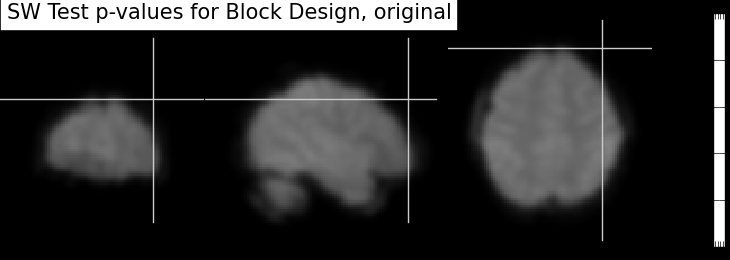
\includegraphics[scale=0.42]{block_normality_test}
\end{subfigure}%
\begin{subfigure}{.4\textwidth}
  \centering
  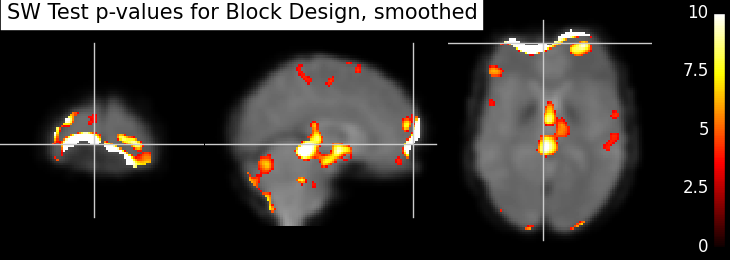
\includegraphics[scale=0.42]{smoothed_block_normality_test}
\end{subfigure}
\begin{subfigure}{.52\textwidth}
  \centering
  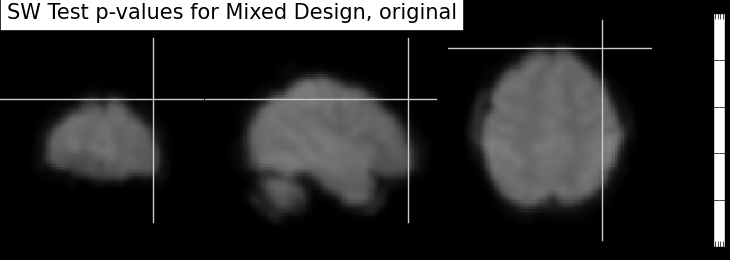
\includegraphics[scale=0.42]{mixed_normality_test}
\end{subfigure}%
\begin{subfigure}{.4\textwidth}
  \centering
  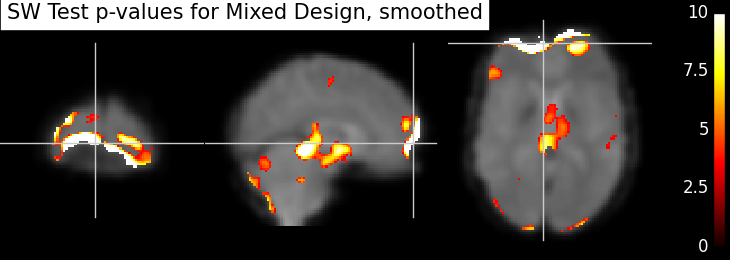
\includegraphics[scale=0.42]{smoothed_mixed_normality_test}
\end{subfigure}
\begin{subfigure}{.52\textwidth}
  \centering
  
\includegraphics[scale=0.42]{mixed_dct_normality_test}
\end{subfigure}%
\begin{subfigure}{.4\textwidth}
  \centering
  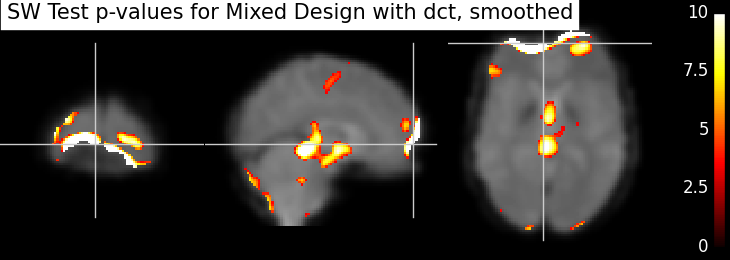
\includegraphics[scale=0.42]{smoothed_mixed_dct_normality_test}
\end{subfigure}
\caption{SW Test for Three Linear Models\label{fig:swtest}}
\end{figure}

The bright areas in the plots means errors in that area don't follow normal 
distribution. We can see that data before smoothed seems to have a lot of 
areas that don't follow normal distribution. After smoothing, the plots look 
much better. They show that only some of the areas are without normality. 
This makes sense because there should be significant points for anatomy.





